% %%%%%%%%%%%%%%%%%%%%%%%%%%%%%%%%%%%%%%%%%%%%%%%%%%%%%%%%%%%%%%%%%%%%%%%%%%%%%%%%%%%%%%%%%%%%
\section{Our approach}
\label{sec:our_approach}

\begin{figure*}[ht!]
\centering
\subfigure[SDG - First Iteration]{
\centering
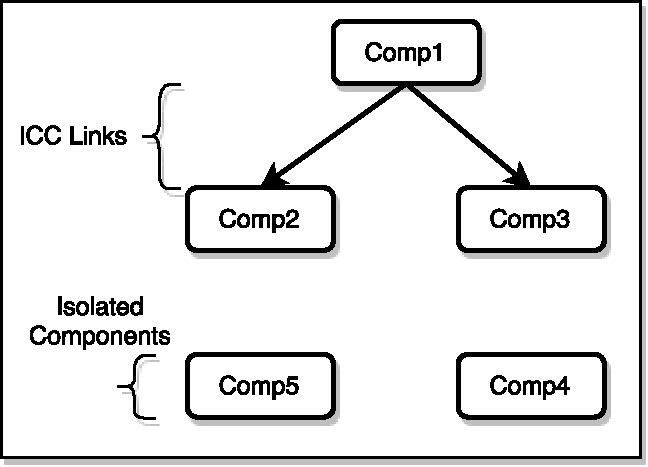
\includegraphics[scale=0.47]{SDG1}
\label{fig:sdg1}
}%
~%Nothing
\subfigure[SDG - Second Iteration]{
\centering
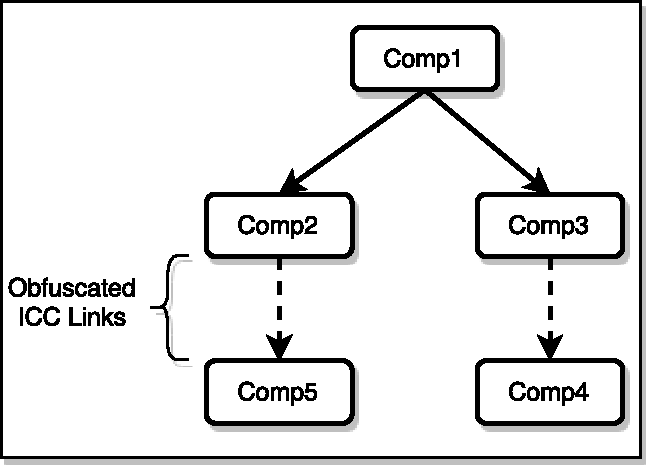
\includegraphics[scale=0.47]{SDG2}
\label{fig:sdg2}
}%
\caption{SDG during the first and second iteration. Comp: Component}
\label{fig:sdg}

\end{figure*}

During a normal execution of an Android app, the control transfers between various components based on certain user or system events. In order to trigger a specific piece of code inside an app, it is important to provide the exact user/system events in a specific order to make it follow the target path. We take a slightly different approach based on isolating target execution paths from within the app and executing them; thereby avoiding to rely on user/system events. Target execution paths are isolated by means of a slice extraction mechanism that leverages backward program slicing across various components of the app.  

\subsection{Slice Extraction}

Backward code slicing is a static analysis technique that identifies the data flow to a certain variable \textit{v} at point \textit{p} in the program while tracking the code in backward direction. In the process it identifies all the code instructions \textit{I} which directly or indirectly affect the value of \textit{v} at point \textit{p}. This set of instructions \textit{I} is called a backward slice. An important property of a backward slice is that it can execute independently of the rest of the program. 

We leverage this property of the backward slice in our approach. Our backward slicing mechanism starts from a target point and traverses the code in backward direction until it reaches an entry point in the app. Instructions corresponding to each target point are marked accordingly and extracted from the program to be refined and executed separately. In simple apps, a backward slice may belong to a single app component. However, the complexity of apps these days demands for more inter component communication. Therefore, approaches based on extracting slices from only a single component might miss critical information passed through ICC.  

\subsection{Inter-Component Communication}

Our approach extends backward slicing across multiple app components. We build a System Dependency Graph (SDG) before starting slice extraction. A SDG is a representation of the program highlighting the inter-connectivity and program flow among various components. Figure~\ref{fig:sdg} provides a simplified representation of a SDG. The \textit{nodes} in the SDG represent components which are connected to each other with directed \textit{edges} where the direction shows the flow of execution from one component to the other. A SDG also provides information about the nature of the components, \textit{i.e.}, activity, service, broadcast receiver, etc. This information is not shown in the figure where we simply refer to them as Comp\textit{X}. The backward slicing assisted by the SDG then extracts slices which may contain instructions from multiple components. 

\iffalse
\begin{figure}[ht!]
\centering
\lstinputlisting[language=Java,label={lst:test1}]{listings/slice.java}
\label{fig:slices}
\caption{Extracted and Refined Slice}
\label{fig:slices}
\end{figure}
\fi

\lstinputlisting[language=Java,label={lst:slices}, caption={Extracted and Refined Slice}]{listings/slice.java}

%Listing \ref{fig:outact} and \ref{fig:inact} show code snippets taken from DroidBench \cite{droidbenchpage} suite. It is an open test suite for evaluating the effectiveness of taint-analysis tools. It is, basically, a collection of several  apps which leak sensitive data exploiting different Android features (like Android activity lifecycle, callback, thread, ICC, etc\ldots). Even if it is mainly intended for a different purpose (the evaluation of taint-analysis tools), in the following we used an example app from Droidbench (the ones which uses ICC for malicious behavior) to describe and demonstrate the effectiveness of our approach. We used the Dexguard \cite{dexguardpage} tool to obfuscate the interesting apps using different techniques like Java reflection and string encryption. Then, instead of looking for a flow between source and sink methods, our goal is to automatically extract the malicious behavior, which involves ICC mechanism, from the obfuscated app.

Our approach uses an iterative mechanism which works in a CreateSDG-ExtractSlice-Execute cycle. Each phase in this cycle provides input for the next phase. SDGs help in extracting slices across multiple components and extracted slices simplify execution of target points in the app. Similarly, the execution phase helps in resolving obfuscation and dynamic code updates which leads to improved creation of the SDG in the next iteration. Figure~\ref{fig:sdg1} and \ref{fig:sdg2} show a SDG in two iterations. In the first iteration, TeICC finds the obvious non-obfuscated ICC links only. Therefore, the SDG contains Comp4 and Comp5 which are isolated components. The second iteration reveals that the app has obfuscated ICC links from Comp2 to Comp5 and from Comp3 to Comp4 as shown in Figure~\ref{fig:sdg2}. This process carries on until the SDG reaches a stable point. At this stage, all the obfuscated links are resolved and the slices are ready for the final execution to capture and analyze suspicious behavior.

%Listing \ref{fig:outact} and \ref{fig:inact} illustrate two Activities. OutFlowActivity which first gets a sensitive data (the IMEI number, line 7 Listing \ref{fig:outact} ) then send it to the second Activity: InFlowActivity. Finally, it does data exfiltration via the SMS vector (line 9 \ref{fig:inact}. The obfuscation by Dexguard encrypts the string in both Activities (lines 11, 13 and 6, 9) with a call to f.e method passing in as argument the encrypted string. Moreover, Listing \ref{fig:outact} line 13, the call to startActivity method has been replaced with an indirect call via Java reflection mechanism. The Intent is created at line 9, then that intent is exchanged between the two components by first attach the data using putExtra (line 11) method and then by invoking the ICC method startActivity (line 13).

%At the best of our knowledge, static analyzers like IC3 \cite{octeau2015composite} and EPICC \cite{octeau2013effective} will fail because of both encryption and reflection techniques. Moreover, also hybrid approaches proposed in \cite{rasthofer2015harvesting} and \cite{backes2016r} fail as well, because they lack support of ICC.

% As discussed before, all existing approaches \cite{octeau2015composite,octeau2013effective,rasthofer2016harvesting,li2015iccta,backes2016r} fail the analysis because either they can not detect flow between different Android components, or because of its obfuscation. This consideration holds for hybrid approaches like Harvester \cite{rasthofer2016harvesting} and R-Droid \cite{backes2016r} as well. Both of them will also fail in the analysis because they can not properly follow ICC flows. 

Most of the state-of-the-art analysis tools would fail to extract the complete slice in the case of the sample described in \S\ref{sec:prob}. However, TeICC allows the extraction of such data-dependent slices because it can follow the ICC flow across multiple components. Listing \ref{lst:slices} shows the resulting slice extracted and refined by TeICC; it shows the corresponding aggregated Java code to ease the understanding. 
%TeICC performs backward slicing starting from a MOI looking for data-dependency. The instructions which are linked with the  MOI are added during the slicing process. Finally, only the instructions which participate in the computation of the target arguments in the MOI are included in the resulting slice, Listing \ref{fig:slices}.

\subsection{Slice Execution}

The extracted slices are put together in one or more resultant components where the irrelevant instructions are removed as shown in Listing~\ref{lst:slices}. Similarly, the \texttt{AndroidManifest.xml} file is also modified to include entries for these resultant components and remove irrelevant ones. The enriched app is then assembled and signed. The flow of the app is hijacked using a stub code so that it executes the resultant component after it is launched. The app is then installed and run on a real device or emulator. The target slice is executed once the resultant component is started. Similarly for each extracted slice, a resultant component is added to the app. The app is observed during execution of the resultant components to capture the target behavior of the app. 

% Android apps are composed of various components where the execution moves from one component to another when it receives certain user or system events. In order to trigger a specific piece of code inside an application, an exact environment needs to be provided. An exact environment may include a number of things, such as a specific OS, specific libraries, real device or emulator, internet connectivity, specific date and time, specific user/system events and so on, depending upon the app. Therefore, different apps require different execution environments. Providing a generic environment which could work with every application is not feasible. To overcome this problem, our new approach is based on removing the environment dependency required for triggering instead of providing the environment. We try to modify the application in such a way that it no more requires triggers from the outside world to execute specific portions of the code. In the following subsections, we provide a step wise explanation of our approach.

% \subsection{Slice Extraction and Categorization}


% In order to reach a specific point in the code, the application must be executed in a such way that it takes the path from an entry point to the target point. Therefore, it is important to identify the path from the entry point to the target. To a larger extent, such path can be identified in an application using some static analysis techniques. Our targeted dynamic triggering solution is also backed by static analysis. In the static analysis phase, a static analyzer identifies the targets in the application. The static analyzer is then used to perform backward slicing of the application to extract the paths composed of code statements starting at an entry point and leading to the identified target. These are the code statements which directly or indirectly influence the instruction in the target code line. Table \ref{tab:single_method_slice} shows an example of a slice. In order to facilitate further analysis, we divide the execution paths/code slices into different categories.

% %In this case, we use a modified version of SAAF (Static Android Analysis Framework) as a static analyzer.

% \textbf{SingleMethod:} Depending upon the depth and the position of the target code line, a slice may contain code statements from one or multiple methods. A single method slice is one which contains statements belonging to only one method. Table \ref{tab:single_method_slice} shows an example of a single method slice where all the statements belong to the \texttt{onCreate} method of the \texttt{wap.syst.activity} class. The first column in the table represents the slice \textit{ID}. Each slice is assigned a unique ID starting from zero, which increments for each new slice corresponding to a new target. The next three columns, \textit{TLine\#}, \textit{TClass} and \textit{TMethod}, represent the target line number, target class and target method, respectively. The column \textit{CClass} represents the class containing the current code line, whereas, the corresponding method is represented by column \textit{CMethod}. The last column contains the code lines including their line numbers and instructions.

% \todo[inline]{Correct the line numbers in the table}

% \begin{table*}[t!]
% \centering
% \caption{Single Method Slice}
% \label{tab:single_method_slice}

% \scriptsize

% \begin{tabular}{|c|c|c|c|c|c|p{6cm}|}
% \hline
% \textbf{ID} & \textbf{TLine\#} & \textbf{TClass} & \textbf{TMethod} & \textbf{CClass} & \textbf{CMethod} & \textbf{CodeLine} \\
% \hline
% \hline

% 0 & 19 & \texttt{wap.syst.activity} & onCreate & \texttt{wap.syst.activity} & onCreate & \texttt{59: move-result-object v1}\\
% 0 & 19 & \texttt{wap.syst.activity} & onCreate & \texttt{wap.syst.activity} & onCreate & \texttt{55: const-string v12, class}\\
% 0 & 19 & \texttt{wap.syst.activity} & onCreate & \texttt{wap.syst.activity} & onCreate & \texttt{52: invoke-virtual {v9, v10}, Ljava/util/Properties;->load(Ljava/io/InputStream;)V}\\
% 0 & 19 & \texttt{wap.syst.activity} & onCreate & \texttt{wap.syst.activity} & onCreate & \texttt{48: invoke-direct {v9}, Ljava/util/Properties;-><init>()V}\\
% 0 & 19 & \texttt{wap.syst.activity} & onCreate & \texttt{wap.syst.activity} & onCreate & \texttt{46: new-instance v9, Ljava/util/Properties;}\\
% 0 & 19 & \texttt{wap.syst.activity} & onCreate & \texttt{wap.syst.activity} & onCreate & \texttt{42: move-result-object v10}\\
% 0 & 19 & \texttt{wap.syst.activity} & onCreate & \texttt{wap.syst.activity} & onCreate & \texttt{38: const/high16 v13, 0x7f05}\\
% 0 & 19 & \texttt{wap.syst.activity} & onCreate & \texttt{wap.syst.activity} & onCreate & \texttt{59: move-result-object v12}\\
% \hline

% \end{tabular}
% \end{table*}


% \textbf{MultipleMethods:} A more usual case will be a multiple method slice which is composed of multiple methods and contains transitions from one method to the other at specific points. Where a single method slice can be triggered fairly easily, the multiple method slices are hard to trigger as the transition might be dependent upon some user/system events or a particular state of some environment variables. Figure \ref{fig:multiple_method_slice} shows an example of a composite slice. The blocks represent methods and the arrows represent transitions from one method to anther method. A slice starts with an \textit{entrypoint} method and ends at a \textit{target} method. The control flows through a number of \textit{intermediate} methods before reaching the target. In Figure \ref{fig:multiple_method_slice}, the methods which are part of the target slice are encapsulated in a box and shaded grey.



% %\begin{figure}[h!]
% %\centering
% %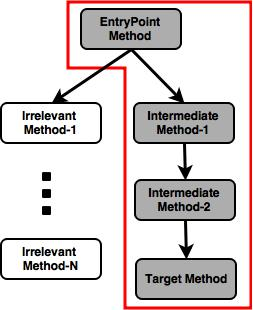
\includegraphics[scale=0.6]{MultipleMethodSlice}
% %\caption{Multiple Method Slice}
% %\label{fig:multiple_method_slice}
% %\end{figure}

% \begin{figure*}[t!]
% \centering
% \subfigure[Multiple Method Slice]{
% \centering
% 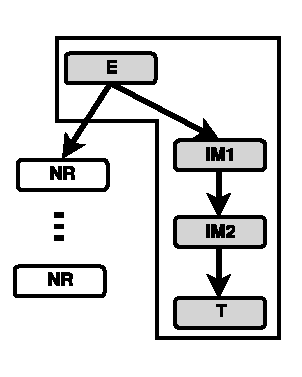
\includegraphics[scale=0.7]{MultipleMethodSliceTExeD.pdf} %[width=.25\textwidth]
% \label{fig:multiple_method_slice}
% }
% ~%Nothing
% \subfigure[Inline Slices]{
% \centering
% 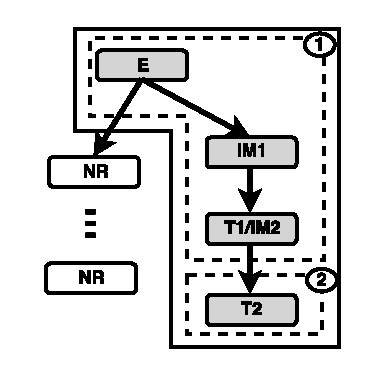
\includegraphics[scale=0.7]{InlineSlicesTExeD.pdf}
% \label{fig:inline_slices}
% }
% ~%Nothing
% \subfigure[Composite Slice]{
% \centering
% 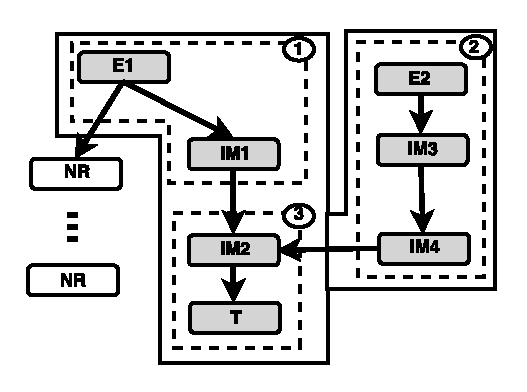
\includegraphics[scale=0.7]{CompositeSliceTExeD.pdf}
% \label{fig:composite_slice}
% }
% \caption{Slice Categories; \textit{E}: Entrypoint Method, \textit{T}: Target Method, \textit{IM}: Intermediate Method, \textit{NR}: Non-relevant Method}
% \label{fig:slice_categories}
% \end{figure*}


% \textbf{InlineSlice:} Inline slices are those slices where one slice is a sub-slice of the other slice. In this case, the targets lie on the same execution path. Therefore, such slices can be triggered in one execution. Figure\ref{fig:inline_slices} shows two such inline slices where the slice encapsulated in the dashed box \circled{1} is a sub-slice of the slice encapsulated in the solid box. The target of first is slice \textit{T1} which serves as an intermediate method for the target \textit{T2}. This can be the case where the target slices represent dynamic class loading and reflection APIs. Usually, additional code is loaded using dynamic class loading APIs and its methods are invoked using reflection APIs. Ideally, this should be a perfect case of inline slices.

% %\begin{figure}[h!]
% %\centering
% %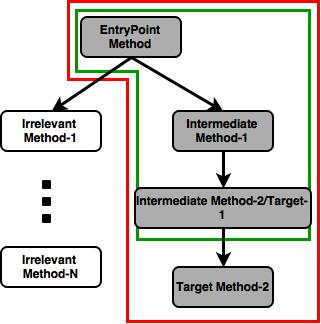
\includegraphics[scale=0.6]{InlineSlices}
% %\caption{Inline Slices}
% %\label{fig:inline_slices}
% %\end{figure}



% \textbf{CompositeSlice:} A target code line, usually an API call, may contain more than one parameters where the flow of information to these parameters could be through different execution paths. Therefore, the corresponding target slice is a combination of multiple distinct slices. Slices corresponding the same target code line combine together to form a composite slice encapsulated in a solid box as shown in Figure\ref{fig:composite_slice}.

% %A backward slice in an application corresponds to a specific pattern where a pattern can be an API call with a specific parameter. Therefore, an API call having multiple interesting parameters would form multiple patterns and thus, result in multiple slices. The next step is to find such slices for each API call invokation instance. There is a unique \textit{ID} for every pattern. However, slices with different \textit{ID}s can be dealt with together if they correspond to the same target code line. Slices corresponding the same target code line combine together to form a composite slice encapsulated in a red box as shown in Figure\ref{fig:composite_slice}.

% %\begin{figure}[h!]
% %\centering
% %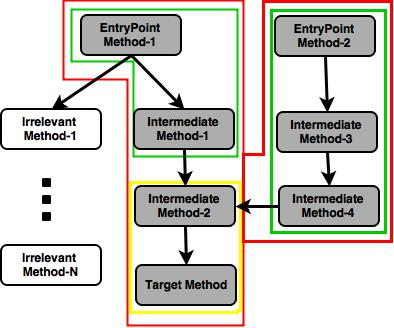
\includegraphics[scale=0.6]{CompositeSlice}
% %\caption{Composite Slice}
% %\label{fig:composite_slice}
% %\end{figure}

% To make things simpler, a composite slice is divided into multiple sub-slices. Among these slices, the common and uncommon portions are separated. Since all these slices end up at the same target line, the latter portion of these slices is more likely to be the common portion, called \textit{CommonSlice} which is encapsulated in the dashed box \circled{3} in Figure\ref{fig:composite_slice}. The uncommon portions in these slices are treated as separate slices, called \textit{PartialSlice}s. In Figure\ref{fig:composite_slice}, partial slices are encapsulated in dashed boxes \circled{1} and \circled{2}. Separation of these slices helps in a making sure that \textit{PartialSlice}s get executed before the \textit{CommonSlice} in this case.

% %Where does the uncommon portion come from? Is it the same method? Or different? If different, whether coming from some eventListener or normal method? Deal the uncommon portions of the slice as different slices. Internally connected using the duplicate/stitch method. N from the outside,
% %MainActivity->PartialSlice1
% %return->MainActivity->ParticalSlice2
% %return->MainActivity->CommonSlice



% %\subsection{Critical Points Identification}
% \subsection{Analyzing Transitions}

% In a multiple method slice, the statements belong to more than one methods and may belong to more than one classes where the transitions from one method to another method can be an explicit one or an implicit one. The identification of such transition points and their nature in the slice are essential in triggering the app along the target slice.

% \begin{lstlisting}[language=java, label={lst:m1tom2}, caption={method1 to method2}]
% .method public method1()V
%  .registers 1
%  .prologue
%  .line 19
%  invoke-virtual {p0}, Ldisi/unitn/targettriger/testapp/MainActivity;->method2()V
%  .line 20
%  return-void
%  .end method
% \end{lstlisting}

% \begin{lstlisting}[language=java, label={lst:m2tom1}, caption={method2 to method1}]
%  .method public method2()V
%  .registers 1
%  .prologue
%  .line 24
%  return-void
%  .end method
% \end{lstlisting}

% In Android apps, the transition of control flow from one method to another can be of various types. Apart from the simple direct method calls in Android apps, various components are started (their corresponding callback methods are called) using Intents. An intent is a message in the Android system which may or not specify a target and describes the operation to be performed. It can be used to launch an Activity (calling the \texttt{startActivity()} method), start a Service (calling \texttt{startService()}) and stimulate a BroadcastReceiver (calling the \texttt{broadcastIntent()}) \ref{}[Developer's guide], etc. Intents can be both explicit, where the target component and methods are specified in the call, and implicit, where the target is not specified in the call. Listing \ref{lst:m1tom2} to Listing \ref{lst:startActivitytoonCreate} show examples of such transitions. In all these cases, no additional external events are required to stimulate the transition from one method to the other. In Listing \ref{lst:m1tom2}, \texttt{method1()} directly calls \texttt{method2()} at line 5. The control returns to \texttt{method1} in line 5 of \texttt{method2()} as shown in Listing \ref{lst:m2tom1}. Similary, Line 16 in Listing \ref{lst:startActivitytoonCreate} represents a transitions to another Activity made through a call to the \texttt{startActivity()} method and providing the information through an intent.


% \begin{lstlisting}[language=java, label={lst:startActivitytoonCreate}, caption={Starting an activity}]
%  .method protected onCreate(Landroid/os/Bundle;)V
%  .registers 4
%  .param p1, "savedInstanceState"    # Landroid/os/Bundle;
%  .prologue
%  .line 15
%  invoke-super {p0, p1}, Landroid/support/v7/app/ActionBarActivity;->onCreate(Landroid/os/Bundle;)V
%  .line 16
%  const v1, 0x7f030017
%  invoke-virtual {p0, v1}, Ldisi/unitn/targettriger/testapp/MainActivity;->setContentView(I)V
%  .line 18
%  new-instance v0, Landroid/content/Intent;
%  const-class v1, Ldisi/unitn/targettriger/testapp/SecondActivity;
%  invoke-direct {v0, p0, v1}, Landroid/content/Intent;-><init>(Landroid/content/Context;Ljava/lang/Class;)V
%  .line 19
%  .local v0, "intent":Landroid/content/Intent;
%  invoke-virtual {p0, v0}, Ldisi/unitn/targettriger/testapp/MainActivity;->startActivity(Landroid/content/Intent;)V
%  .line 22
%  return-void
% .end method
% \end{lstlisting}


% However, there are transition points which require either system events or user events to get triggered. These are the critical points in a slice which need to be taken care off to reach the targets. This step identifies these critical points and puts them into appropriate categories for necessary actions. Currently, we divide the transition points into different categories, i.e., method calls, return-to-caller, Intents, UI events, system events. Listings \ref{lst:onCreatetoonClick} and \ref{lst:XtoonBatteryLow} provide examples of a UI event listener and a system event listener, respectively. These methods are only called when a specific event, that they are waiting for, happens.

% \begin{lstlisting}[language=java, label={lst:onCreatetoonClick}, caption={onCreate to onClick}]
% onCreate(){
% //Click Listener. UI event
%   onClick(){
%     //onClick handler code
%   }
% }
% \end{lstlisting}

% \begin{lstlisting}[language=java, label={lst:XtoonBatteryLow}, caption={X to onBatteryLow}]
% anyClass extends BroadcastReceiver(){
%   //Battery Low Listener. System event
%   onBatteryLow(){
% 	//onBatteryLow handler code
%   }
% }
% \end{lstlisting}

% %Return/New Call: Differenciate between a new call and return to the same method. Add explanation of return-to-caller. E.g., Method1->Method2->Method1 most probably will be a return to Method1 from Method2.}



% \subsection{Creating Duplicates for Event Listeners}

% %\todo[inline]{Some event listeners can be called directly, while some others may not be. We may not need duplication in cases when event listeners can be called directly.}

% %Identify whether a method is an event listener or not: By comparing it with a list of all event listeners

% %Analyze the parameters and accordingly generate similar mock parameters in the duplicate method

% %Keep track of the duplicate methods so that an event listener is not duplicated more than once.

% %Q: How to do with the event listener is in another activity? Whether to get an instance of that activity and call the corresponding duplicate method or launch that activity and then call the corresponding duplicate method?

% Among the mentioned categories, some of them, i.e., method calls, return-to-caller and intents (sent within the app), do not require any instrumentation for ensuring transition from one method to the other in our approach. The app's own logic can be used to trigger such transitions. However, in order to trigger the later two, appropriate events are required depending upon the nature of the event listeners. Since we use a different approach for triggering, i.e., making the triggering environment-independent rather than providing the exact environment, we modify the app's APK in such a way that external events are not required for stimulating the app along the target execution paths.

% %\begin{figure*}[htp]
% %  \centering
% %  \subfloat[Before Duplication and %Stitching]{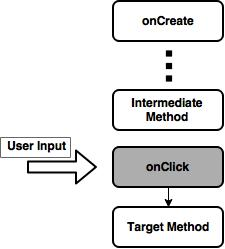
\includegraphics[scale=0.6]{DuplicationNStitching-1}\label{subfig:dup_stitch_1}}
% %  \subfloat[After Duplication and %Stitching]{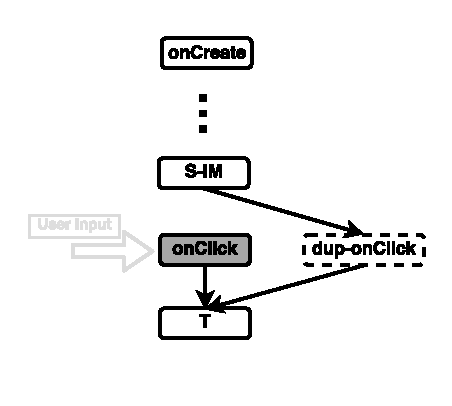
\includegraphics[scale=0.6]{DuplicationNStitching-2}\label{subfig:dup_stitch_2}}
% %  \label{fig:dup_stitch}
% %  \caption{Original app's flow Vs Modified app's flow}
% %\end{figure*}

% In order to do so, ordinary methods which are duplicates of the event listeners are created and instrumented inside in the app's smali files. Figure \ref{subfig:dup_stitch_1} shows a sample control flow of an application which starts at the \textit{onCreate} method and passes through some intermediate methods. At the \textit{onClick} method, it requires a UI event to proceed the execution along the target path. Dependability on the UI event (and for that matter on any system event too) is removed using a duplicate method of the event listener represented by dashed rectangle as shown in Figure \ref{subfig:dup_stitch_2}. So, these duplicate methods can be called to ensure stimulating the functionality coded inside the event listeners without providing any external events. The duplicate methods are named so that their names portray a relation between the duplicate method and the original event listener. Moreover, the system also keeps tracks of the duplicate methods so that an event listener is not duplicated more than once.

% %\todo[inline]{Need to design a naming convention for the duplicate methods so that they provide enough information about the original event listener.}

% \begin{figure}[t!]
% \centering
% \subfigure[Original]{
% \centering
% 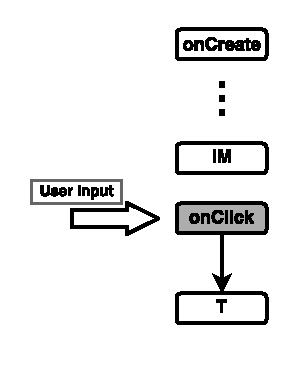
\includegraphics[scale=0.6]{DuplicationNStitching-1.pdf} %[width=.25\textwidth]
% \label{subfig:dup_stitch_1}
% }
% ~%Nothing
% \subfigure[Intrumented]{
% \centering
% 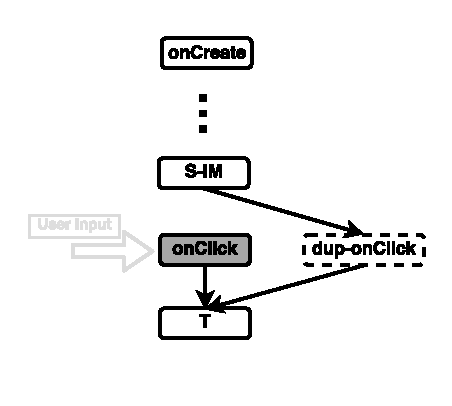
\includegraphics[scale=0.6]{DuplicationNStitching-2.pdf}
% \label{subfig:dup_stitch_2}
% }
% \caption{Original app's flow Vs Instrumented app's flow}
% \label{fig:dup_stitch}
% \end{figure}

% \subsection{Stitching: Inter-Method Control Flow}

% The control flow of an application from its entry point towards a given target is not always spontaneous, but it has to go through a number of user and system events at appropriate positions. Therefore, the extracted slice misses connectivity where the next method in the slice is an event listener. The connectivity at these critical points is dependent upon the UI/system events corresponding to the event listener. In order to remove this dependency, we connect the (duplicates of) event listeners to their preceding methods in the control flow and we call this process \textit{Stitching}. The stitching process consists of insertion of an direct method call to the (duplicate) event listener method in the method which precedes it according to the information provided by the extracted code slice in the first step.

% \begin{lstlisting}[language=java, label={lst:stitching}, caption={Stitching the Duplicate Methods}]
% ...
% //Inserted Method call
% invoke-virtual {p0, v0}, Ldisi/unitn/targettriger/testapp/MainActivity;->duplicate-onClick()V
% ...
% \end{lstlisting}

% Listing \ref{lst:stitching} shows an example of such an inserted method call. Location of the stitches depends upon the position of the event listener in the slice. Event listeners at the start of a slice (event listener as an entry point of the slice) would require their duplicate methods to be stitched with the \textit{onCreate} in MainActivity of the app. Also, there can be cases where all the statements that form a slice are from a single event listener. Such cases are handled similarly. However, when there is an event listener in the middle or at the end of the slice, a stitch needs to be placed in the method immediatedly preceding the event listener in the slice. Stitching ensures that the functionality coded insided an event listener is executed without the occurence of the required event as shown in Figure \ref{subfig:dup_stitch_2}.




% \subsection{Ensuring Intra-Method Control Flow}

% %Note: Remember Opaque predicates
% %We don't need to go for Opaque predicates, rather we follow the path in the code slice.


% Stitching accounts for the inter-method flow of the app execution. However, the intra-method flow an app execution might be hindered by the app's logic itself, such as the presence of conditional statements. TExeDroid traverses each method in the slice and extracts information on whether and how a conditional statement might affect the target. For instance, a conditional statement might be irrelevant to the target statement or it's \texttt{if}/\texttt{else}/both clause might have an effect on the target statement. In case, where the target statement depends upon the \texttt{if} clause only, the triggering system instrument the conditional statement to be always true, and vice versa. However, when execution of both the \texttt{if} and \texttt{else} clauses might affect the target statement, our system deals them in two separate runs of execution, one each for the \texttt{if} and \texttt{else} clause. Listings \ref{lst:conditional_statement} the instrumentation performed for the above mentioned cases.

% \noindent\begin{minipage}{.25\textwidth}
% \begin{lstlisting}[language=java, caption={\texttt{if} clause},label={lst:if}]
% ...
% if(true){
% 	//if clause
% }
% else{
% 	//else clause
% }
% ...

% TARGET.call();
% \end{lstlisting}
% \end{minipage}\hfill
% \begin{minipage}{.25\textwidth}
% \begin{lstlisting}[language=java, caption={\texttt{else} clause}, label={lst:else}]
% ...
% if(false){
% 	//if clause
% }
% else{
% 	//else clause
% }
% ...

% TARGET.call();
% \end{lstlisting}
% \end{minipage}





% However, the relation between the conditional statement and the actual statement can not always be that simple. In cases where there is no relation between the variable used in the conditional statement and those used in the actual statement, simply making the condition \texttt{true} works fine. However, if the variables in the conditional statement have a direct effect on the actual statement, the previous solution may or may not work, specially in cases where these values are taken from the outside world. In cases where the variable used in the condition is also used in the target statement, we instrument the conditional statement in three different ways, i.e., replacing the condition by a boolean \texttt{true}, \texttt{false} and change the value of the variable such that the condition becomes \texttt{true}. This instrumentation ensures the execution of the target statement, however, this still does not guarantee an accurate solution for the problem when the values of the variable used are taken from the outside world at runtime, such as through an SMS or from the Internet. For instance, a variable \textit{x} which takes its value from an incoming SMS and its value is zero/null otherwise. If there is a conditional statement such as \texttt{if(x)} followed by a target statement such as \texttt{sendTextMessage(x,..);}, we will never know the exact value of the \textit{x} and making it true doesn't solve the issue completely. However, cases where conditional statements are like \texttt{if(x==y)} are followed by the target statement can be solved, where \textit{y} is another variable/constant whose value is known. Similar reasoning applies to other conditional statements as well, such as \texttt{switch} statement.

% \todo[inline]{Basic block concept in the above para}
% \todo[inline]{Commenting invoke statements where the control diverts to non-relevant method.}

% \iffalse

% \subsection{Logging Critical Info}

% \textbf{General:} The purpose of dynamic analysis is to know the behavior of an app. Target-Trigger, however, focuses only on the execution of certain paths leading to specific APIs. In order to know the runtime values of the parameters passed to these target APIs, we instrument the app with hooks placed before every target API call. These hooks make sure to capture the runtime values of such parameters of interest.

% \textbf{StaDyna:} In case of coupling T-TDroid with StaDyna (a tool for resolving the targets of reflection and dynamic class loading) as a triggering solution, StaDyna requires additional information to identify the correct position of the called methods in the method call graph. Stadyna generates a complete method call graph of the application taking into consideration the runtime calls to reflection APIs and the code which is loaded dynamically. For generating a complete method call graph, it is important to know the exact position of new nodes that are to be added to the method call graph. This additional information is required only when the reflection/dynamic class loading calls are inside the duplicated event listeners. There, in order to capture this additional information, T-TDroid places hooks in the duplicated even listeners which provide information about their actual counterparts.
% \fi

% \subsection{Execution along the target path}

% Once the instrumentation related to a particular slice is over, TExeDroid reassembles the app from its Smali files and signs it. The repackaged app is then installed on a target device or emulator. The instrumentation explained in this section above makes sure that the application follows the target path (for a specific slice), once launched, without requiring any external UI or system event. Instrumentation is performed for a particular target (one target execution path at a time) and, hence, it must be repeated for each target in the app. Therefore, TExeDroid works in an instrument-repackage-launch cycle where the number of the instrument-repackage-launch cycles is less than or equal to the number of target statements in the app. In case an app having inline slices, multiple slices are triggered in the same instrument-repackage-launch cycle.



% %######################################################################################


% \iffalse

% We use a precise and efficient methodology for targeted test case generation.

% \begin{itemize}
% \item Method Call Graph generation
% \item Target paths extraction
% \item Node categorization in the target paths (Callback methods, UI events, System events, other methods)
% \item Symbolic execution of methods where necessary
% \item Use the above info generating an accurate chain of actions (test cases) which leads to target in the give app
% \end{itemize}

% We use symbolic execution for targeted test case generation. Symbolic execution usually suffers from the path explosion problem. It is an expensive method of test case generation and takes a lot of time. To cater these problems, our symbolic execution engine is based on a Method Call Graph (MCG) of the application. The MCG is used to guide the symbolic execution engine and prune unnecessary exploration. A coarse view of the whole process is show in Figure \ref{fig:work_flow}.

% \begin{figure}[h]
% \centering
% 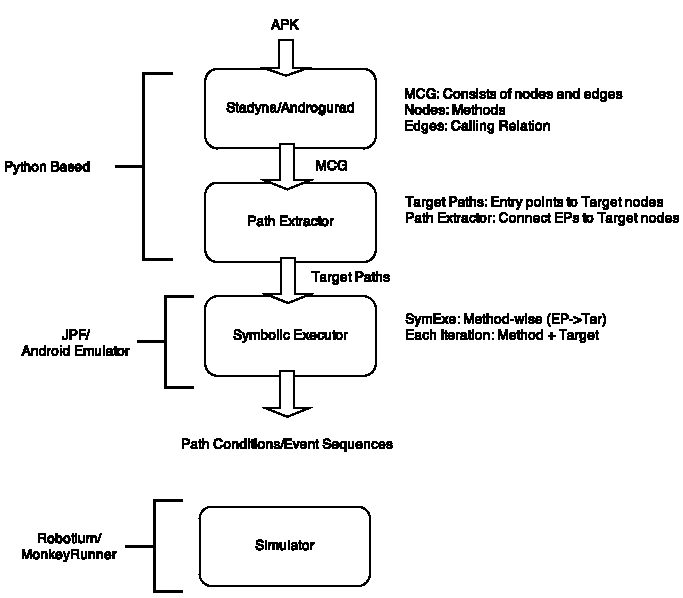
\includegraphics[width=14cm]{TTeCGAT-Workflow}
% \caption{TTeCGAT Work Flow}
% \label{fig:work_flow}%
% \end{figure}

% \subsection{Stitched Method Call Graph}

% An MCG consists of nodes and edges where nodes represent methods and edges represent a calling relation between the methods. The MCG is constructed from the Dalvik bytecode of the application. Android apps are mostly event (both user and system) driven and contain callback methods of the framework which are implemented by the app developer. Generally, the flow of an app may vary from one execution to another based on the received user and system events. Moreover, Android app components such as activities and services are started using intent messages rather than a direct method call. Therefore, a statically generated MCG consists of several disconnected MCGs. These disconnected MCGs need to be stitched together, based on sources of targets of intent messages, to form a Stitched Method Call Graph.

% The nodes in the MCG are divided into three categories. 1) Entry point (EP) 2) Intermediate nodes 3) Target nodes. EPs correspond to the methods from where an application can be stimulated. Target nodes represent those methods which contain the target code (line, API, method, etc.) for which we want to generate test cases. Intermediate nodes are those methods which construct the path from EPs to target nodes.


% \subsection{Extraction of Target Paths: Reducing the search space}

% After construction of the MCG and identification of the EPs and target nodes, the next step to extract the paths, which start from the EPs and lead to the target node through one or more intermediate nodes. Sometimes, the EP may directly be connected to the target node without having any intermediate nodes in between. Moreover, a node can be an EP as well as a target node at the same time. Target paths are extracted from the MCG by traversing it from a target node in backward until an EP is reached. There can be cases where more than one target paths, starting from the same or different EPs, are extracted for the same target. Moreover, a non-deterministic interleaving of callback methods based on user and system events makes it harder to find out the exact flow of events which lead to a certain target node. In addition, there may be methods which may not be part of the original path which leads to the target node, but effect the state of app in such a manner that is essential for reaching the target node. So, it is important to include these supportive methods in the search space. Here, the search space is essentially reduced using the MCG.

% \subsection{Symbolic Execution}

% Our Symbolic execution engine is guided by the extracted target paths. We perform a two-level symbolic execution of the app. 1) A method-wise symbolic execution for all the nodes in the target path. The aim of the symbolic execution is to generate test cases for each method which can lead to the next method on the specific target path. So, each node has a method name and target inside that method for which symbolic execution engine tries to generate test cases. The test cases generated for one method are fed to the symbolic execution engine of the next method which has a newer target corresponding to the next method in the target path. 2) The second level of symbolic execution tries to find out the combination of these methods which lead to the target node. So, at the stage a more concise list of methods is identified which helps in generating a possible test case for the app. This process continues until a possible test case (a sequence of events) is generated which can stimulate the application from an EP to the target. This process is repeated for all the target paths (paths from EPs to targets).

% \subsection{Stimulating Applications}

% At end of the symbolic execution process, we get one or more test cases for each target path, which are converted to concrete event sequences. These event sequences are then fed to a simulator (such as Robotium, MonkeyRunner, etc.) which exercises the original application on an Android emulator or real device.

% \fi
